\documentclass[12pt,]{article}
\usepackage[utf8]{inputenc}
\usepackage[T1]{fontenc}
\usepackage{mathptmx}
\usepackage{geometry}
\usepackage{mathtools}
\usepackage[english]{babel}
\usepackage{graphicx}
\usepackage{stackengine}
\usepackage[os=win]{menukeys}
\usepackage{hyperref}
\usepackage{minted}
\usepackage{xcolor}
\usepackage{tikz}
\usepackage[yyyymmdd,hhmmss]{datetime}
\usepackage{etoolbox}

\patchcmd{\thebibliography}{\section*{\refname}}{}{}{}

\newcommand{\ShowOsVersion}{
	\immediate\write18{\unexpanded{foo=`uname -sro` && echo "${foo}" > tmp.tex}}
	\input{tmp}\immediate\write18{rm tmp.tex}
}

\newcommand{\ShowTexVersion}{
	\immediate\write18{\unexpanded{foo=`pdflatex -version | head -n1 | cut -d' ' -f1,2` && echo "${foo}" > tmp.tex}}
	\input{tmp}\immediate\write18{rm tmp.tex}
}

\addto\captionsenglish{\renewcommand{\contentsname}{Daftar Isi}}

\hypersetup{
	colorlinks=true, %set true if you want colored links
	linktoc=all,     %set to all if you want both sections and subsections linked
	linkcolor=blue,  %choose some color if you want links to stand out
	urlcolor=blue,	 %url color
}

\geometry{
	legalpaper,
	left=15mm,
	right=10mm,
	top=10mm,
	bottom=15mm,
}

\title{\Large \bf
	License and Patent Claim Draft\\
	\small{(Mid-Testing Stage)}
}

\author{Achmadi ST MT}

\date{}

\hypersetup{citecolor=black}

\definecolor{LightGray}{gray}{0.95}

%\pagecolor[rgb]{0.1,0.1,0.1}
%\color[rgb]{1,1,1}

\begin{document}
	\maketitle
	\thispagestyle{empty}
	
	\vspace*{600pt}
	\noindent Seluruh konten dalam dokumen ini mengacu kepada pengembangan unit Audiometri di \textit{commit} terakhir:\\
	\url{https://github.com/VibrasticLab/pikoakustik/commit/fa1db9a040644eab3fd033c1f8c43e28af1f0ebf}.\\
	
	\noindent This report written using: \\
	OS : \ShowOsVersion \\
	TeX : \ShowTexVersion \\
	Update: {\today} at \currenttime \\
	
	%%%%%%%%%%%%%%%%%%%%%%%%%%%%%%%%%%%%%%%%%%%%%%%%%%%%%%%%%%%%%%%%%
	
	\newpage
	\tableofcontents
	
	%%%%%%%%%%%%%%%%%%%%%%%%%%%%%%%%%%%%%%%%%%%%%%%%%%%%%%%%%%%%%%%%%
	
	\newpage
	\section{Software/Firmware}
	
	Berikut akan dijabarkan beberapa aspek dari sisi software/firmware yang dijalankan di hardware.
	Seluruh klaim pada aspek ini dalam bentuk klaim kode sumber (\textit{source-code}) dan tidak terbatas hanya \textit{binary} akhir.
	Referensi untuk fungsi-fungsi implementasi dapat ditemukan di source-tree di alamat:
	\begin{itemize}
		\item (STM32) \url{https://github.com/VibrasticLab/pikoakustik/tree/stm32f401re_3pin/firmware}
		\item (ESP8266) \url{https://github.com/VibrasticLab/pikoakustik/tree/stm32f401re_3pin/esp8266}
	\end{itemize}
	
	\subsection{Libraries}
	Disini akan dijabarkan pengunaan pustaka (libraries) yang digunakan dalam pengembangan.
	Seluruh pustaka disini berupa kode sumber implementasi dan API (\textit{Application Programming Interface})
	di luar implementasi dan perbaikan (\textit{patch}) yang dilakukan oleh pihak peneliti disini.
	
	Penjabaran ini perlu mengingat pustaka tersebut dikembangankan oleh pihak lain dan telah memiliki klaim lisensi sendiri.
	Sehingga secara otomatis pihak peneliti disini \textbf{tidak bisa mengklaim} pustaka tersebut.
	
	\begin{itemize}
		\item \textbf{GNU GCC ARM}. Merupakan sekumpulan \textit{toolchain} dan pustaka untuk kompilasi source-code ke binary untuk chip ARM.
		Dikembangan oleh ARM Limited dengan lisensi yang digunakan adalah GPL versi 3.0\\
		\url{https://developer.arm.com/open-source/gnu-toolchain/gnu-rm}
		
		\item \textbf{ChibiOS/RT}. Merupakan sekumpulan pustaka yang berisi implementasi dan API abstraksi untuk chip ARM seri Cortex-M.
		Dikembangkan oleh Giovanni Di Sirio dengan lisensi yang digunakan adalah GPL versi 3.0 dan Apache versi 2.0\\
		\url{https://www.chibios.org/dokuwiki/doku.php}
		
		\item \textbf{FatFS}. Merupakan sekumpulan pustaka yang berisi implementasi dan API abstraksi untuk FAT16/FAT32 \textit{filesystem}.
		Pustaka ini digunakan untuk menangani berkas-berkas teks yang disimpan di \textit{memory-card}.
		Dikembangkan oleh Elm ChanN dengan lisensi yang digunakan adalah BSD license.\\
		\url{http://elm-chan.org/fsw/ff/00index_e.html}
		
		\item \textbf{ESP-Open-SDK}. Merupakan sekumpulan \textit{toolchain} dan pustaka untuk kompilasi source-code ke binary untuk platform ESP8266/EX.
		Dikembangan oleh Tensilica Inc. dan Espressif Inc. dengan lisensi yang digunakan adalah GPL versi 2.0\\
		\url{https://github.com/pfalcon/esp-open-sdk}
		
		\item \textbf{esp\_mqtt}. Merupakan sekumpulan pustaka yang berisi implementasi protocol MQTT Client untuk ESP8266/EX.
		Dikembangkan oleh Tuan PM dengan lisensi yang digunakan adalah MIT License.\\
		\url{https://github.com/tuanpmt/esp_mqtt}
	\end{itemize}

	\subsection{Audio}
	
	Berikut dijabarkan beberapa klaim terhadap referensi metode/algoritma terkait fitur Audio/Tone.
	
	\subsubsection{Tone Generation}
	
	Referensi persamaan untuk \textit{tone generation}.
	Aspek klaim adalah pola persamaan dan seluruh definisi konstanta yang digunakan,
	terkecuali objek struktur konfigurasi I2S.
	
	Referensi fungsi/implementasi ini ini dapat dilihat di berkas
	\href{https://github.com/VibrasticLab/pikoakustik/blob/stm32f401re_3pin/firmware/ht_audio.c#L69-L100}{firmware/ht\_audio.c:69-100}

	\subsubsection{Tone Play}
	
	Referensi metode untuk \textit{tone playing}.
	Aspek klaim adalah durasi dan flow metode, terkecuali objek struktur konfigurasi I2S.

	Referensi fungsi/implementasi ini ini dapat dilihat di berkas
	\href{https://github.com/VibrasticLab/pikoakustik/blob/stm32f401re_3pin/firmware/ht_audio.c#L102-L110}{firmware/ht\_audio.c:102-110}

	\subsubsection{L/R Control}
	
	Referensi metode untuk kendali channel kiri-kanan.
	Aspek klaim adalah flow metode, terkecuali nomor pin pada chip STM32.
	
	Referensi fungsi/implementasi ini ini dapat dilihat di berkas:
	\begin{itemize}
		\item \href{https://github.com/VibrasticLab/pikoakustik/blob/stm32f401re_3pin/firmware/ht_audio.c#L112-L115}{firmware/ht\_audio.c:112-115}
		\item \href{https://github.com/VibrasticLab/pikoakustik/blob/stm32f401re_3pin/firmware/ht_audio.c#L117-L120}{firmware/ht\_audio.c:117-120}
		\item \href{https://github.com/VibrasticLab/pikoakustik/blob/stm32f401re_3pin/firmware/ht_audio.c#L122-L125}{firmware/ht\_audio.c:122-125}
	\end{itemize}
	
	\newpage
	\subsection{Serial Commands}
	
	Berikut dijabarkan beberapa klaim terhadap referensi metode/algoritma terkait fitur Serial Commands yang dapat diakses melalu jalur USB-CDC.
	
	\subsubsection{Testing}
	Perintah untuk menjalankan rutin testing baik untuk komunikasi serial dan audio
	\begin{minted}[frame=lines,framesep=2mm,fontsize=\small,bgcolor=LightGray]{bash}
ch> test [0|1]
	\end{minted}

	Referensi fungsi/implementasi ini ini dapat dilihat di berkas
	\href{https://github.com/VibrasticLab/pikoakustik/blob/stm32f401re_3pin/firmware/ht_comm.c#L49-L96}{firmware/ht\_comm.c:49-96}

	\subsubsection{Audio: Zero}
	Perintah untuk menjalankan rutin testing tone pada 0 dBV.
	\begin{minted}[frame=lines,framesep=2mm,fontsize=\small,bgcolor=LightGray]{bash}
ch> zero [0/1]
	\end{minted}

	Referensi fungsi/implementasi ini ini dapat dilihat di berkas
	\href{https://github.com/VibrasticLab/pikoakustik/blob/stm32f401re_3pin/firmware/ht_comm.c#L104-L125}{firmware/ht\_comm.c:104-125}

	\subsubsection{Audio: Max}
	Perintah untuk menjalankan rutin testing tone pada dBV maximum.
	\begin{minted}[frame=lines,framesep=2mm,fontsize=\small,bgcolor=LightGray]{bash}
ch> max [0/1]
	\end{minted}

	Referensi fungsi/implementasi ini ini dapat dilihat di berkas
	\href{https://github.com/VibrasticLab/pikoakustik/blob/stm32f401re_3pin/firmware/ht_comm.c#L131-L152}{firmware/ht\_comm.c:131-152}
	
	\subsubsection{Audio: Min}
	Perintah untuk menjalankan rutin testing tone pada dBV minimum.
	\begin{minted}[frame=lines,framesep=2mm,fontsize=\small,bgcolor=LightGray]{bash}
ch> min [0/1]
	\end{minted}

	Referensi fungsi/implementasi ini ini dapat dilihat di berkas
	\href{https://github.com/VibrasticLab/pikoakustik/blob/stm32f401re_3pin/firmware/ht_comm.c#L158-L179}{firmware/ht\_comm.c:158-179}

	\subsubsection{Audio: Tone}
	Perintah untuk menjalankan rutin testing tone pada skala frekuensi dan amplitud tertentu.
	\begin{minted}[frame=lines,framesep=2mm,fontsize=\small,bgcolor=LightGray]{bash}
ch> tone <0/1> <freq> <ampl>
	\end{minted}

	Referensi fungsi/implementasi ini ini dapat dilihat di berkas
	\href{https://github.com/VibrasticLab/pikoakustik/blob/stm32f401re_3pin/firmware/ht_comm.c#L185-L277}{firmware/ht\_comm.c:185-277}
	
	\subsubsection{Audio: Sing}
	Perintah untuk menjalankan rutin testing tone skala tertinggi hingga terendah pada skala frekuensi tertentu.
	\begin{minted}[frame=lines,framesep=2mm,fontsize=\small,bgcolor=LightGray]{bash}
ch> sing <0/1> <freq>
	\end{minted}
	
	Referensi fungsi/implementasi ini ini dapat dilihat di berkas
	\href{https://github.com/VibrasticLab/pikoakustik/blob/stm32f401re_3pin/firmware/ht_comm.c#L233-L280}{firmware/ht\_comm.c:233-280}

	\subsubsection{Audio: Speaker Test}
	Perintah untuk menjalankan rutin testing speaker dengan dua tone berurutan.
	Referensi tone di berkas \textbf{ht\_audio.c}.
	\begin{minted}[frame=lines,framesep=2mm,fontsize=\small,bgcolor=LightGray]{bash}
ch> sptest <0/1/2>
	\end{minted}
	
	Referensi fungsi/implementasi ini ini dapat dilihat di berkas
	\href{https://github.com/VibrasticLab/pikoakustik/blob/stm32f401re_3pin/firmware/ht_comm.c#L286-L298}{firmware/ht\_comm.c:286-298}
	
	\subsubsection{MMC: List Files}
	Perintah untuk menjalankan menampilkan daftar file yang tersimpan di MMC.
	Referensi metode MMC di berkas \textbf{ht\_mmc.c}.
	\begin{minted}[frame=lines,framesep=2mm,fontsize=\small,bgcolor=LightGray]{bash}
ch> ls
	\end{minted}
	
	Referensi fungsi/implementasi ini ini dapat dilihat di berkas
	\href{https://github.com/VibrasticLab/pikoakustik/blob/stm32f401re_3pin/firmware/ht_comm.c#L306-L311}{firmware/ht\_comm.c:306-311}
	
	\subsubsection{MMC: Show File}
	Perintah untuk menjalankan menampilkan isi file yang tersimpan di MMC pada nomer tertentu.
	Referensi metode MMC di berkas \textbf{ht\_mmc.c}.
	\begin{minted}[frame=lines,framesep=2mm,fontsize=\small,bgcolor=LightGray]{bash}
ch> cat [N]
	\end{minted}
	
	Referensi fungsi/implementasi ini ini dapat dilihat di berkas
	\href{https://github.com/VibrasticLab/pikoakustik/blob/stm32f401re_3pin/firmware/ht_comm.c#L317-L324}{firmware/ht\_comm.c:317-324}
	
	\subsubsection{MMC: Test Write}
	Perintah untuk menjalankan rutin test Read/Write di MMC.
	Referensi metode MMC di berkas \textbf{ht\_mmc.c}.
	\begin{minted}[frame=lines,framesep=2mm,fontsize=\small,bgcolor=LightGray]{bash}
ch> mmc
	\end{minted}
	
	Referensi fungsi/implementasi ini ini dapat dilihat di berkas
	\href{https://github.com/VibrasticLab/pikoakustik/blob/stm32f401re_3pin/firmware/ht_comm.c#L330-L336}{firmware/ht\_comm.c:330-336}
	
	\subsubsection{MMC: Show Contents}
	Perintah untuk menjalankan rutin test File Read di MMC.
	Referensi metode MMC di berkas \textbf{ht\_mmc.c}.
	\begin{minted}[frame=lines,framesep=2mm,fontsize=\small,bgcolor=LightGray]{bash}
ch> mmcat
	\end{minted}
	
	Referensi fungsi/implementasi ini ini dapat dilihat di berkas
	\href{https://github.com/VibrasticLab/pikoakustik/blob/stm32f401re_3pin/firmware/ht_comm.c#L342-L348}{firmware/ht\_comm.c:342-348}
	
	\subsubsection{MMC: Check MMC}
	Perintah untuk menjalankan rutin test \textit{filesystem} di MMC.
	Referensi metode MMC di berkas \textbf{ht\_mmc.c}.
	\begin{minted}[frame=lines,framesep=2mm,fontsize=\small,bgcolor=LightGray]{bash}
ch> mmcat
	\end{minted}
	
	Referensi fungsi/implementasi ini ini dapat dilihat di berkas
	\href{https://github.com/VibrasticLab/pikoakustik/blob/stm32f401re_3pin/firmware/ht_comm.c#L354-L360}{firmware/ht\_comm.c:354-360}
	
	\subsubsection{IOT: MQTT Subscribe}
	Perintah untuk menjalankan rutin test subscribe via MQTT.
	Referensi metode MMC di \textit{source-tree} proyek \textbf{esp8266dev}.
	\begin{minted}[frame=lines,framesep=2mm,fontsize=\small,bgcolor=LightGray]{bash}
ch> sub
	\end{minted}
	
	Referensi fungsi/implementasi ini ini dapat dilihat di berkas
	\href{https://github.com/VibrasticLab/pikoakustik/blob/stm32f401re_3pin/firmware/ht_comm.c#L368-L374}{firmware/ht\_comm.c:368-374}
	
	\subsubsection{IOT: MQTT Publish}
	Perintah untuk menjalankan rutin test Publish via MQTT.
	Referensi metode MMC di \textit{source-tree} proyek \textbf{esp8266dev}.
	\begin{minted}[frame=lines,framesep=2mm,fontsize=\small,bgcolor=LightGray]{bash}
ch> pub
	\end{minted}
	
	Referensi fungsi/implementasi ini ini dapat dilihat di berkas
	\href{https://github.com/VibrasticLab/pikoakustik/blob/stm32f401re_3pin/firmware/ht_comm.c#L380-L386}{firmware/ht\_comm.c:380-386}
	
	\newpage
	\subsubsection{IOT: MQTT Send HTTP JSON}
	Perintah untuk menjalankan rutin test kirim JSON hasil ke server via HTTPS.
	Referensi metode MMC di \textit{source-tree} proyek \textbf{esp8266dev}.
	\begin{minted}[frame=lines,framesep=2mm,fontsize=\small,bgcolor=LightGray]{bash}
ch> send
	\end{minted}
	
	Referensi fungsi/implementasi ini ini dapat dilihat di berkas
	\href{https://github.com/VibrasticLab/pikoakustik/blob/stm32f401re_3pin/firmware/ht_comm.c#L392-L399}{firmware/ht\_comm.c:392-399}
	
	\subsubsection{IOT: MQTT Send MQTT Result Log}
	Perintah untuk menjalankan rutin test kirim JSON hasil ke server via HTTPS.
	Referensi metode MMC di \textit{source-tree} proyek \textbf{esp8266dev}.
	\begin{minted}[frame=lines,framesep=2mm,fontsize=\small,bgcolor=LightGray]{bash}
ch> log <freq> <ampl> [TRUE/FALSE]
	\end{minted}
	
	Referensi fungsi/implementasi ini ini dapat dilihat di berkas
	\href{https://github.com/VibrasticLab/pikoakustik/blob/stm32f401re_3pin/firmware/ht_comm.c#L405-L416}{firmware/ht\_comm.c:405-416}

	\subsection{Button dan LED}
	
	Berikut dijabarkan beberapa klaim terhadap referensi metode/algoritma terkait fitur antar muka tombol dan indikator LED.
	
	\subsubsection{Start Audiometri}
	
	Untuk memulai proses pengukuran Audiometri, pengguna melakukan tekan tombol dengan suatu urutan.
	Aspek klaim disini adalah flow urutan tombol dan LED untuk memulai proses pengukuran audiometri.
	Urutan tombol dan led:
	
	\begin{figure}[!ht]
		\centering
		\includegraphics[width=350pt]{images/ledbutton_step}
		\caption{Urutan tombol dan LED interaksi proses Audiometri}
	\end{figure}

	Urutan untuk memulai proses audiometri adalah:
	
	\begin{enumerate}
		\item Saat kondisi \textit{idle}, LED pada posisi ini akan berkedip lambat.
		
		\item Tekan salah satu dari 3 tombol yang sebaris.
		
		\item LED terdekat dengan tombol menyala
		
		\item Tekan tombol lain selain tombol sebelumnya.
		
		\item LED sebelum nya akan mati dan LED Hijau menyala.
		Ini adalah kondisi standby/siap
		
		\item Tekan tombol lain selain dua tombol sebelumnya.
		
		\item LED pada posisi ini akan berkedip cepat dan LED lainnya akan mati.
		Proses Audiometri dimulai.
		
	\end{enumerate}

	Proses Audiometri akan selesai ditandai dengan LED pada langkah 1 atau 7 kembali berkedip lambat.
	
	\newpage
	Referensi untuk proses ini tersedia di berkas:
	\begin{itemize}
		\item \href{https://github.com/VibrasticLab/pikoakustik/blob/stm32f401re_3pin/firmware/ht_exti.c#L75-L82}{firmware/ht\_exti.c:75-82}
		\item \href{https://github.com/VibrasticLab/pikoakustik/blob/stm32f401re_3pin/firmware/ht_exti.c#L87-L95}{firmware/ht\_exti.c:87-95}
		\item \href{https://github.com/VibrasticLab/pikoakustik/blob/stm32f401re_3pin/firmware/ht_exti.c#L102-L139}{firmware/ht\_exti.c:102-139}
		\item \href{https://github.com/VibrasticLab/pikoakustik/blob/stm32f401re_3pin/firmware/ht_exti.c#L145-L182}{firmware/ht\_exti.c:145-182}
		\item \href{https://github.com/VibrasticLab/pikoakustik/blob/stm32f401re_3pin/firmware/ht_exti.c#L188-L225}{firmware/ht\_exti.c:188-225}
		\item \href{https://github.com/VibrasticLab/pikoakustik/blob/stm32f401re_3pin/firmware/ht_metri.c#L136-L307}{firmware/ht\_metri.c:136-307}
		\item \href{https://github.com/VibrasticLab/pikoakustik/blob/stm32f401re_3pin/firmware/main.c#L48-L126}{firmware/main.c:48-126}
	\end{itemize}

	\subsubsection{Input Audiometri}
	
	Referensi untuk interaksi pengguna saat proses audiometri berjalan.
	Aspek klaim disini adalah flow proses tombol dan respon LED saat.
	Urutan tombol dan led:
	
	\begin{figure}[!ht]
		\centering
		\includegraphics[width=350pt]{images/ledbutton_input}
		\caption{Urutan tombol dan LED untuk memulai}
	\end{figure}

	Flow yg dimaksud adalah:
	\begin{enumerate}
		\item Pastikan LED berkedip cepat sebagai indikator proses Audiometri sedang berjalan.
		
		\item Setiap LED pada grup ini akan berkedip satu kali secara berurutan.
		Salah satu diantara nya akan memberikan bunyi Tone
		
		\item Tekan satu Tombol pada grup ini sesuai LED yang menyala bersamaan dengan bunyi Tone terdengar.
		
		\item LED pada grup ini menyala salah satu. Hijau jika benar (LED, Tombol, dan Tone sesuai) dan Merah jika salah.
	\end{enumerate}

	Pengguna akan mengulangi aksi serupa hingga proses Audiometri selesai dan unit kembali \textit{idle} ditandai LED pada poin satu berkedip lambat
	
	Referensi untuk proses ini tersedia di berkas:
	\begin{itemize}
		\item \href{https://github.com/VibrasticLab/pikoakustik/blob/stm32f401re_3pin/firmware/ht_exti.c#L102-L139}{firmware/ht\_exti.c:102-139}
		\item \href{https://github.com/VibrasticLab/pikoakustik/blob/stm32f401re_3pin/firmware/ht_exti.c#L145-L182}{firmware/ht\_exti.c:145-182}
		\item \href{https://github.com/VibrasticLab/pikoakustik/blob/stm32f401re_3pin/firmware/ht_exti.c#L188-L225}{firmware/ht\_exti.c:188-225}
		\item \href{https://github.com/VibrasticLab/pikoakustik/blob/stm32f401re_3pin/firmware/ht_metri.c#L136-L307}{firmware/ht\_metri.c:136-307}
		\item \href{https://github.com/VibrasticLab/pikoakustik/blob/stm32f401re_3pin/firmware/ht_metri.c#L309-L337}{firmware/ht\_metri.c:309-337}
		\item \href{https://github.com/VibrasticLab/pikoakustik/blob/stm32f401re_3pin/firmware/main.c#L48-L126}{firmware/main.c:48-126}
	\end{itemize}

	\newpage
	\subsection{Memory Card Saving}
	
	Berikut dijabarkan beberapa klaim terhadap referensi metode/algoritma terkait fitur \textit{file-saving} di memory card.
	
	\subsubsection{MMC LED Indicator}
	
	Metode ini digunakan menunjukkan Memory Card (MMC) tersedia dan siap digunakan menggunakan LED indikator utama.
	Jika LED berkedip lambat, maka MMC siap dan unit idle.
	Jika LED berkedip cepat 2 kali setiap 2 detik, maka unit idle dengan tanpa MMC atau MMC tidak siap.
	
	Referensi untuk proses ini tersedia di berkas:
	\begin{itemize}
		\item \href{https://github.com/VibrasticLab/pikoakustik/blob/stm32f401re_3pin/firmware/ht_mmc.c#L168-L214}{firmware/ht\_mmc.c:168-214}
		\item \href{https://github.com/VibrasticLab/pikoakustik/blob/stm32f401re_3pin/firmware/ht_mmc.c#L216-L279}{firmware/ht\_mmc.c:216-279}
		\item \href{https://github.com/VibrasticLab/pikoakustik/blob/stm32f401re_3pin/firmware/main.c#L48-L126}{firmware/main.c:48-126}
	\end{itemize}
	
	\subsubsection{String Parser}
	
	Metode ini digunakan memisahkan string atau array karakter dengan pemisah berupa spasi, karakter NULL, atau karakter \textit{non-alphanumeric}.
	
	Referensi fungsi/implementasi ini ini dapat dilihat di berkas
	\href{https://github.com/VibrasticLab/pikoakustik/blob/stm32f401re_3pin/firmware/ht_mmc.c#L74-L94}{firmware/ht\_mmc.c:74-94}
	
	\subsubsection{File Format}
	
	Metode ini digunakan menulis hasil record pengukuran Audiometri di setiap jawaban pada setiap frekuensi dan amplitudo.
	Termasuk aspek klaim adalah penamaan pola nama file dan format konten file teks yang disimpan.
	
	Referensi untuk proses ini tersedia di berkas:
	\begin{itemize}
		\item \href{https://github.com/VibrasticLab/pikoakustik/blob/stm32f401re_3pin/firmware/ht_mmc.c#L522-L601}{firmware/ht\_mmc.c:552-601}
		\item \href{https://github.com/VibrasticLab/pikoakustik/blob/stm32f401re_3pin/firmware/ht_mmc.c#L603-L653}{firmware/ht\_mmc.c:603-653}
		\item \href{https://github.com/VibrasticLab/pikoakustik/blob/stm32f401re_3pin/firmware/ht_mmc.c#L655-L695}{firmware/ht\_mmc.c:655-695}
	\end{itemize}

	\subsection{Wifi Module}
	
	\subsubsection{Wifi Mode Switching}
	
	Metode ini menyediakan mode Wifi sebagai Access Point untuk pengaturan secara wireless
	dan sebagai Wifi Station/Bridge untuk komunikasi antara unit dan server data.
	Pengaturan mode dengan \textit{slide-switch}.
	
	Referensi untuk proses ini tersedia di berkas:
	\begin{itemize}
		\item \href{https://github.com/VibrasticLab/pikoakustik/blob/stm32f401re_3pin/esp8266/user/wifi_sap.c}{esp8266/wifi\_sap.c}
		\item \href{https://github.com/VibrasticLab/pikoakustik/blob/stm32f401re_3pin/esp8266/user/wifi_sta.c}{esp8266/wifi\_sta.c}
		\item \href{https://github.com/VibrasticLab/pikoakustik/blob/stm32f401re_3pin/esp8266/user/wifi_sta.c}{esp8266/user.c}
	\end{itemize}

	\subsubsection{Serial Input MQTT Transfer}
	
	Metode untuk merespon perintah serial untuk pengiriman data via protokol MQTT.
	
	Referensi fungsi/implementasi ini ini dapat dilihat di berkas
	\href{https://github.com/VibrasticLab/pikoakustik/blob/stm32f401re_3pin/esp8266/user/drv_uart.c#L343-L364}{esp8266/mqtt\_client.c:343-364}

	\subsubsection{MQTT JSON Data}
	
	Standar format field dan array JSON untuk pertukaran data via TCP/IP dengan protokol MQTT.
	
	Referensi fungsi/implementasi ini ini dapat dilihat di berkas
	\href{https://github.com/VibrasticLab/pikoakustik/blob/stm32f401re_3pin/esp8266/user/mqtt\_client.c}{esp8266/mqtt\_client.c}
	
	\subsubsection{HTTP JSON Data}
	
	Standar format field dan array JSON untuk pertukaran data via TCP/IP dengan protokol HTTP.
	
	Referensi fungsi/implementasi ini ini dapat dilihat di berkas
	\href{https://github.com/VibrasticLab/pikoakustik/blob/stm32f401re_3pin/esp8266/user/drv\_uart.c}{esp8266/drv\_uart.c}
	
	\newpage
	\subsection{Summary}
	
	Berikut rangkuman aspek teknis yang dapat diajukan untuk klaim paten dan lisensi:
	
	\begin{itemize}
		\item Audio
		\begin{enumerate}
			\item Tone Generation
			\item Tone Playing
			\item Left/Right Control
		\end{enumerate}
	
		\item Serial Commands/Interface
		\begin{enumerate}
			\item Testing
			\item Tone Zero
			\item Tone Maximum
			\item Tone Minimum
			\item Tone Play 
			\item Tone Sing
			\item Tone Speaker Test
			\item File List
			\item File Show Content
			\item File Show Content Test
			\item File Read/Write Test
			\item File Read Test
			\item File Check Memory
			\item MQTT Subscribe
			\item MQTT Publish
			\item MQTT Send HTTP
			\item MQTT Log Result
		\end{enumerate}
	
		\item Button-LED Interface
		\begin{enumerate}
			\item Start Audiometri
			\item User input Audiometri
		\end{enumerate}
	
		\item Memory Card
		\begin{enumerate}
			\item MMC Readyness Indicator
			\item Filename String Parser
			\item Text Saving Format
		\end{enumerate}
	
		\item Wifi Module
		\begin{enumerate}
			\item Wifi Mode Switching
			\item Serial Input MQTT
			\item MQTT JSON Data
			\item HTTP JSON Data
		\end{enumerate}
	\end{itemize}

	Total untuk saat ini tersedia 29 aspek teknis di sisi software/firmware yang bisa diajukan klaim.

	\newpage
	\section{Hardware}
	Berikut akan dijabarkan beberapa aspek dari sisi desain hardware,
	terutama desain layout dari papan sirkuit (PCB).
	
	\subsection{Overall Layout}
	
	Klaim pada aspek ini adalah rancangan/desain terkait pola penempatan 
	(layout) komponen untuk interaksi dengan pengguna.
	
	\begin{figure}[!ht]
		\centering
		\includegraphics[width=400pt]{images/layout}
		\caption{Layout penempatan LED/Tombol untuk interaksi dengan pengguna}
	\end{figure}

	Keterangan layout komponen:
	\begin{enumerate}
		\item Tombol untuk proses audiometri
		
		\item LED untuk proses Audiometri
		
		\item LED untuk Benar-Salah di proses Audiometri
		
		\item Tombol reset unit
		
		\item LED indikator mode
		
		\item Slot Memory Card untuk penyimpanan hasil
		
		\item USB untuk antar-muka ke Android/Windows/Linux
		
		\item Jack Audio T-R-S ukuran 3.5mm
	\end{enumerate}

	\newpage	
	\subsection{Handheld Usage}
	
	Klaim pada aspek ini terkait penggunaan unit produk yang \textit{portable}
	dan \textit{handheld} yang ditandai dengan:
	
	\begin{itemize}
		\item Ukuran unit yang secara relatif sama dengan ukuran genggaman 
		tangan (90mm x 60mm)
		
		\item Ditenagai dengan battery Li-Ion yang portabel dan dapat diisi 
		ulang
	\end{itemize}

	\begin{figure}[!ht]
		\centering
		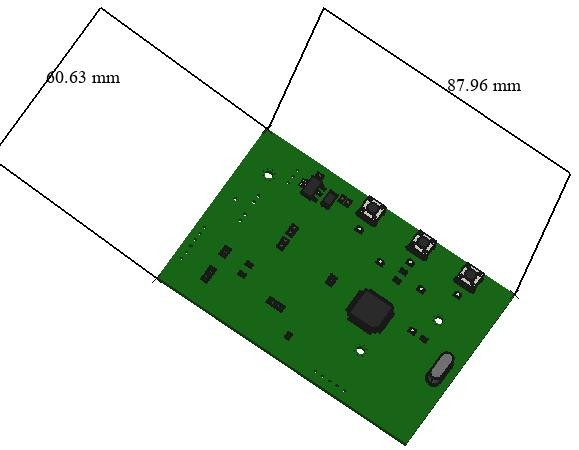
\includegraphics[width=350pt]{images/size}
		\caption{ukuran relatif unit}
	\end{figure}
	
\end{document}